\documentclass{article}

\usepackage[T1]{fontenc}

\usepackage[margin=1.0in]{geometry}
\usepackage{longtable}

\usepackage{amsmath}

\newcounter{example}
\newenvironment{example}[1][]{\refstepcounter{example}\par\medskip
   \noindent \textit{Example~\theexample. #1} \rmfamily}{\medskip}

\usepackage{bbm}
\usepackage{booktabs}

\newcommand{\fabs}[1]{\mid {#1} \mid}

\newcommand{\bet}[1]{\llbracket {#1} \rrbracket^{\beta} }
\usepackage{stmaryrd}
\usepackage{graphicx}
\usepackage{tikz}
\usepackage{wrapfig}
\usepackage{makecell}

% \usepackage{mathabx}
\usepackage{amssymb,forest}

\usepackage{float}
\usepackage{MnSymbol}
\newlength\q
\newlength\smallCol
\newlength\argsLen
\setlength\q{\dimexpr .5\textwidth -2\tabcolsep}
\setlength\smallCol{\dimexpr .15\textwidth}
\setlength\argsLen{\dimexpr .2\textwidth}


\newcommand{\lto}{\mathbin{\to}}
\usepackage{booktabs}
\usepackage{enumitem} 
\usepackage{array}% for extended column definitions
\usepackage{graphicx}
\usepackage{verbatim}
\usepackage{tabto}
\newcommand{\ov}[2]{\ensuremath{\overset{\cdot {#2} \cdot}{#1}}}
\newcommand{\imp}{\rightarrow}

\usepackage{xstring}
\usepackage[german]{babel}
\usepackage[utf8]{inputenc}

\usepackage{lipsum}
\usepackage{listings}

\newcommand{\tcr}[1]{\textcolor{red}{#1}}

\definecolor{palegreen}{rgb}{0.9,1,0.9}
\usepackage[most]{tcolorbox}
\tcbset{
    frame code={}
    center title,
    left=0pt,
    right=0pt,
    top=0pt,
    bottom=0pt,
    colback=palegreen,
    colframe=white,
    width=\dimexpr\textwidth\relax,
    enlarge left by=0mm,
    boxsep=5pt,
    arc=0pt,outer arc=0pt,
    after={\par\vspace{\baselineskip}\noindent},
  }
  \renewcommand{\arraystretch}{2}
\usepackage{color}

\definecolor{dkgreen}{rgb}{0,0.6,0}
\definecolor{gray}{rgb}{0.5,0.5,0.5}
\definecolor{mauve}{rgb}{0.58,0,0.82}
\definecolor{lightpink}{rgb}{1.0,0.9,0.9}
\definecolor{darkblue}{rgb}{0,0,0.4}

\usepackage{hyperref}

\hypersetup{colorlinks=true,linkcolor=darkblue,citecolor=darkblue}



\lstset{frame=tb,
  language=Java,
  aboveskip=3mm,
  belowskip=3mm,
  showstringspaces=false,
  columns=flexible,
  basicstyle={\small\ttfamily},
  numbers=none,
  numberstyle=\tiny\color{gray},
  keywordstyle=\color{blue},
  commentstyle=\color{dkgreen},
  stringstyle=\color{mauve},
  breaklines=true,
  breakatwhitespace=true,
  tabsize=3
}
\lstset{language=Python}

\title{Gralog Console Manual}

\author{Felix Herron\\\texttt{felix.herron@tu-berlin.de}
  \and Roman Rabinovich\\ \texttt{roman.rabinovich@tu-berlin.de}
\and Adrian Alic\\ \texttt{adrian.alic@campus.tu-berlin.de}}

\date{\today}

\begin{document}

\maketitle


\begin{abstract}
Gralog is a visual tool for working with graphs, logics, games,
transition systems and other structures based on undirected and
directed graphs. It can create, load, save and edit graphs in
various formats.

The key focus of Gralog is simplicity of use and a short time of
learning how to use it.

A special property of Gralog is that it helps the developer to write
programmes for graphs in any language capable of working with
pipes. Gralog visualises the run of the programme and can keep track
of values of user defined variables.

The interaction between Gralog and the external programme is
performed by a simple, but powerful protocol. In the first version
we implemented a library for Python that simplifies the interaction
and abstracts away the use of pipes. This paper describes the
protocol and the library, the External Programming Module (EPM). This
includes documentation of methods and classes pertaining to the
EPM and code examples for how to use these.
\end{abstract}

\section{Documentation and Installation}

You can download Gralog from \url{https://github.com/gralog/gralog}.

First, make sure that Java version at least 10 is installed on your
machine. (Currently, version 11 does not seem to work with Gralog.)

On Linux and Mac OS you can install it by

\begin{tcolorbox}
  cd..

  ./install-linux.sh
\end{tcolorbox}

This compiles Gralog in directory \texttt{~/gralog} (which is created
if necessary) or in the directory you give the script as a parameter:

\begin{tcolorbox}
  ./install-linux.sh /path/to/gralog
\end{tcolorbox}

Then a symbolic link to the script starting Gralog is created in
\texttt{/usr/bin}. For this, the installer asks the user for the admin
password. If you do not have it, just give three times a wrong
password: only the symbolic link part will be skipped.

Furthermore, the installer tries to install Python modules \emph{networkx} and
\emph{python-igraph} with \emph{pip}. If \emph{pip} is not installed,
it tries to install it. If Python is not installed, the installation
stops at this point (however, Python is installed by default on Linux
machines and on Macs). If on your machine by default, \emph{networkx}
and \emph{python-igraph} must be
installed to a directory you do not have writing rights for, the
installer asks for the \texttt{sudo} password.

You can skip the installation of the Python part giving the installer
parameter \texttt{-n} like this:

\begin{tcolorbox}
  ./install-linux.sh /path/to/gralog -n
\end{tcolorbox}
or
\begin{tcolorbox}
  ./install-linux.sh -n /path/to/gralog
\end{tcolorbox}

Finally, you can call the installer with parameter \texttt{-u}:

\begin{tcolorbox}
  ./install-linux.sh /path/to/gralog -u
\end{tcolorbox}
to let \emph{pip} try to install the modules locally. (This
corresponds to calling \texttt{pip install --user <module>}.)

On Windows Gralog is not tested yet. You can try to install it by
running

\begin{tcolorbox}
  gradlew.bat
\end{tcolorbox}
in the Gralog root directory. This compiles Gralog if necessary and
runs it. The \texttt{jar} file is
\texttt{./build/dist/gralog-fx.jar}. Similarly, on Linux and Mac OS
one can call
\begin{tcolorbox}
  ./gradlew
\end{tcolorbox}


On Windows and on newer Macs it is possible to call the jar file by
just clicking on it.

To use the python part on Windows, you have to install Python and the
libraries \emph{networkx} and \emph{python-igraph} yourself. Then copy
the file
\texttt{./gralog-fx/src/main/java/gralog/gralogfx/piping/scripts/Gralog.py}
to the directory with your Python script or somewhere where Python
will find it.


The documentation can be found in directory \texttt{doc/}. The main
manual file is \texttt{gralog.pdf}. This part is additionally in the
file \texttt{external.pdf}. [TODO: make a general manual, include this
text there.]


\section{Working with the console}

The console is a tool to work with graphs by entering commands rather
than by clicking the mouse buttons. This is especially convenient if
you want to create large subgraphs with a regular pattern.

By default, the console is the frame below the main frame with the
graph. Here, in the bottom line, you can enter commands just like in a
terminal.

\subsection{Lists}

The objects you work with are \emph{lists:} lists of vertices and
lists of edges. We concentrate on vertex lists in this manual, edge
lists behave similarly. Where appropriate, we point out the
differences.

The lists are used to connect them later.


\begin{example}[Running example]
  For example, if one wants to create a perfect matching with $50$
  edges, one way to do that in Gralog is to create two disjoint lists
  of vertices and then connect them by drawing an edge from vertex $i$
  in the first list to vertex $i$ in the second list. Well, for a
  matching we would use a generator (see
  Section~\ref{sec:generators}), but what if we want to add edges such
  that already exiting $100$ vertices build a matching?
  \label{ex:running}
\end{example}


\subsection{Creating lists, (de)selecting elements}

All lists can be created out of the default list of all
vertices and the internal list of all currently selected vertices. The
latter can be made with the mouse in the obvious way or you can write
in the command line:
\begin{tcolorbox}
  select all vertices,
\end{tcolorbox}
\noindent
to select all vertices. By the way, in a similar way, all vertices are
deselected:

\begin{tcolorbox}
deselect all vertices.
\end{tcolorbox}

Now use the selection to create a new list. The corresponding command
is \texttt{filter}: one filters the elements from an existing list
according to certain criteria and saves them into another list. If the
other list already exists, the new elements are appended to it (even
if they are already contained in the target list). 

\begin{tcolorbox}
  filter all selected where no condition to VL1
\end{tcolorbox}

When creating list ids as \texttt{VL1}, keep in mind that the names
must be unique, in particular, it is impossible that a vertex list and
an edge list have the same name.

\subsection{Filter}

Now we created a new list \texttt{VL1} containing all vertices of the
graph. Let us now create a new list that contains only vertices with a
certain property, say those whose colour is blue. We can now use
\texttt{VL1} as a source of vertices.

\begin{tcolorbox}
  filter VL1 where fill color blue to VLblue
\end{tcolorbox}

Now the list \texttt{VLblue} contains all vertices with fill color
\texttt{blue}. Ne create a new list containing all vertices whose fill
color is red. Note in the following example that instead of the
keyword \texttt{where} one can write \texttt{such that} or
\texttt{st}. Note also that instead of \texttt{fill color} it is
possible to use just \texttt{fill}:

\begin{tcolorbox}
  filter VL1 st fill red to VLred
\end{tcolorbox}

The full specification of the filter command is as follows. Note that
Gralog does not distinguish between the upper and the lower cases.


\begin{tcolorbox}[colback=lightpink]
  FILTER <what> WHERE|ST|(SUCH THAT) <parameters> TO <list identifier>
  [ignored trash]
\end{tcolorbox}
 
\noindent where

\begin{tcolorbox}[colback=lightpink]
  \begin{tabular}[H]{rl}
    <what> := &ALL VERTICES | ALL EDGES\\
              &| [ALL ]? SELECTED VERTICES | [ALL ]? SELECTED EDGES\\
              & | <list id> \\[0.3cm]
    <parameters> := &<parameters> <parameters> | <boolean parameter>\\
              & | <fixed range parameter> <value>\\
              &| <numerical parameter> <cmp> <value> \\[0.3cm]
%                    & | FORMULA <integer expression(i)>\\
    <fixed range parameter> := & SHAPE | TYPE | EDGE TYPE | EDGETYPE \\[0.3cm]
    <numerical parameter> := & <integer parameter> | <float
                               parameter> | <string parameter>\\[0.3cm]
    <integer parameter> := & ID | DEGREE | INDEGREE |
                             OUTDEGREE\\[0.3cm]
    <float parameter> := & FILL | FILL COLOR | STROKE | STROKE
                       COLOR\\
                     &| THICKNESS | WIDTH | HEIGHT | SIZE |
                       WEIGHT\\[0.3cm]
    <string parameter> := &LABEL CONTAINS\\
    <boolean parameter> := &NO CONDITION | HAS SELFLOOP | DIRECTED | HAS
                             LABEL\\
              &| LABEL EMPTY | NO LABEL \\
                     &| BUTTERFLY // not implemented yet
  \end{tabular}
\end{tcolorbox}

In other words, we can write something like

\begin{tcolorbox}
  FILTER sourceList ST FILL RED STROKE BLUE SHAPE ELLIPSE DEGREE > 3 TO targetList
\end{tcolorbox}

Let us look at the grammar closer. In \texttt{<what>} there is no
difference between \texttt{ALL SELECTED VERTICES} and \texttt{SELECTED
VERTICES}, the result will be the same. The \texttt{<list id>} is the
name of a list we defined previously, it can be a list of vertices or
a list of edges.

The order of parameters in the parameter list is arbitrary. The list
of parameters cannot be empty. If you do not want any specifications,
choose \texttt{NO CONDITION}. In that case even if other parameters
are given, they are not taken into account and the whole source list
is given. This can be in particular used to duplicate every element in
a list:

\begin{tcolorbox}
  FILTER sourceList ST NO CONDITION TO newList

  FILTER sourceList ST NO CONDITION TO newList
\end{tcolorbox}

In this case \texttt{newList} will contain every element of
\texttt{sourceList} twice. By the way, being in the command line, one
can press $\uparrow$ (the arrow up key) to call previous commands.

Table~\ref{tab:parsAndVals} explains which values the parameters can have.

\begin{table}
  \centering
  \begin{tabular}{p{3cm}|p{5cm}|p{1.8cm}|p{5cm}}
    \textbf{parameter} &  \textbf{possible values} & \textbf{applicable to}  & \textbf{meaning}\\
    \hline
    \texttt{SHAPE}     &  ELLIPSE, RECTANGLE, DIAMOND & vertices& ellipse,
                                                                  rectangle, diamond\\
                       &  SQUARE, CYCLE & vertices & not implemented yet\\
    \hline
    \texttt{STROKE} or \texttt{STROKE COLOR} (synonyms)
                       &  WHITE, BLACK, BLUE, GREEN, RED, GRAY, \mbox{YELLOW},
                         CYAN, MAGENTA, SILVER, MAROON, OLIVE,
                         DARK\_GREEN, PURPLE, TEAL, NAVY, ORANGE
                                                   & both & the colour of the
                                                            border; other
                                                            colours are
                                                            possible as
                                                            properties of
                                                            vertices, but not
                                                            supported by the
                                                            filter
                                                            command\\
    \hline
    \texttt{EDGE TYPE} & SHARP, ROUND, BEZIER & edges & sharp or rounded
                                                        corners or a
                                                        B\'{e}zier curve\\
    \hline
    \texttt{FILL} or \texttt{FILL COLOR} (synonyms)
                       & as for \texttt{STROKE} & vertices & the fill color,
                                                             otherwise as for
                                                             \texttt{STROKE}\\
    \hline
    \texttt{WIDTH}     & float                 & vertices & \tcr{???}\\
    \hline
    \texttt{THICKNESS} & float                 & both\tcr{?} & \textcolor{red}{???}\\
    \hline
    \texttt{HEIGHT}     & float                & vertices  & \textcolor{red}{???}\\
    \hline
    \texttt{SIZE} & float                      & vertices \tcr{?}  & \textcolor{red}{???}\\
    \hline
    \texttt{WEIGHT} & float                      & edges  &
                                                            \textcolor{red}{???}\\
    \hline
    \texttt{ID}      & non-negative integer   & both & the internal unique id of
                                                       the vertex or of the edge\\
    \hline
    \texttt{DEGREE}    & non-negative integer & vertices & the degree of
                                                           the vertex;
                                                           only
                                                           undirected
                                                           edges count\\
    \hline
    \texttt{INDEGREE}    & non-negative integer & vertices & the in-degree of
                                                             the vertex;
                                                             only
                                                             directed
                                                             edges count\\
    \hline
    \texttt{OUTDEGREE}    & non-negative integer & vertices & the out-degree of
                                                              the vertex;
                                                              only
                                                              directed
                                                              edges count\\
    \hline
    \texttt{HAS SELFLOOP}  & no value & vertices & true if the vertex
                                                   has a self-loop\\
    \hline
    \texttt{NO SELFLOOP}  & no value & vertices & true if the vertex
                                                  has no self-loop\\
    \hline
    \texttt{LABEL EMPTY} or \texttt{NO LABEL} (synonyms)
                       & no value & vertices & true if the label is
                                               empty\\
    \hline
    \texttt{LABEL CONTAINS} & string & vertices & true if the label
                                                  contains the given string\\
    \hline
  \end{tabular}
  \caption{Parameters and their values}
  \label{tab:parsAndVals}
\end{table}

\subsection{Sorting the lists}

Before connecting lists of vertices (recall Example~\ref{ex:running})
we probably want to sort them, so that we know what vertex has
number~$i$. The lists can be sorted by

\begin{tcolorbox}[colback=lightpink]
  SORT <list id> <parameter>
\end{tcolorbox}%
where \texttt{parameter} is one of \texttt{LEFTRIGHT},
\texttt{RIGHTLEFT}, \texttt{TOPDOWN}, \texttt{BOTTOMUP}, \texttt{ID
  ASC}, \texttt{ID DECS}, \texttt{LABEL ASC}, \texttt{LABEL DESC}. The
former four parameters imply a sorting according to the corresponding
coordinate of vertices on the screen, \texttt{ID ASC} sorts by the id
in  the ascending order, \texttt{ID DESC} sorts by the id
in  the descending order and \texttt{LABEL} sorts alphabetically
(ascending or descending) by the label. If the labels of two vertices
are equal, the vertices keep their relative order.

\subsection{Operations on lists (before connecting)}

The following operations are currently supported:

\begin{tcolorbox}[colback=lightpink]
  \begin{tabular}[H]{p{7cm}|p{8cm}}
    \textbf{operation}    & \textbf{meaning}\\
    DELETE <list id> & deletes the list, but not the elements of the list from the graph\\

    UNION <source1> <source2> TO <target> & creates the union of \texttt{source1} and \texttt{source2} and stores the result in \texttt{target}\\

    INTERSECTION <list1 id> <list2 id> TO <list3 id> &creates the intersection of \texttt{source1} and \texttt{source2} and stores the result in \texttt{target}\\
    
    DIFFERENCE <source1> <source2> TO <target> & creates the difference of \texttt{source1} and \texttt{source2} and stores the result in \texttt{target}\\
    
    SYMMETRIC DIFFERENCE <source1> <source2> TO <target>  & creates the symmetric difference of \texttt{source1} and \texttt{source2} and stores the result in \texttt{target}\\
    
    COMPLEMENT <list id> TO <target>  & creates the complement of \texttt{list id} and stores the result in \texttt{target}.\\
    
    CONTRACT <vertex list id> | <edge list id> | SELECTED & builds a minor of the graph by contracting the subgraph induced by the elements of the list or by the selected elements (if \texttt{SELECTED} is specified and some elements are selected) to a single vertex. Works for all kinds of graphs. Not implemented yet.\\
    BUTTERFLY CONTRACT <edge list id> & builds a butterfly minor of the graph by butterfly contracting all butterfly contractable edges. On undirected edges the operation has no effect. Not implemented yet.\\

    SUBDIVIDE <edge list id> <$n$> & subdivides every edge from the list $n$ times where $n$ must be a natural number. Directed edges are replaced by directed paths of length $n+1$. Not implemented yet.
  \end{tabular}
\end{tcolorbox}

\subsection{Connecting lists of vertices}

One can either connect one list of vertices to another, which, however, can be the same list, or connect vertices of one list in a certain way. The first is done by the command

\begin{tcolorbox}[colback=lightpink]
  CONNECT <list1> <list2> =<formula> | BICLIQUE | MATCHING
\end{tcolorbox}

The easier case is to use a standard way of connection, for example,

\begin{tcolorbox}[colback=palegreen]
  CONNECT upper lower MATCHING
\end{tcolorbox}
which produces a matching connecting the $i$th vertex of
\texttt{list1} to the $i$th vertex of \texttt{list2}

%%% Local Variables:
%%% mode: latex
%%% TeX-master: "main"
%%% End:

\section{Setting up your External Python Program}
To link your script to Gralog, create a python file and import (all of) it. This is easiest (and \textit{recommended} if you want the provided code snippet to work) if the library and your script are in the same directory - python can be finicky about such things.\\

In the new file you created, paste the following code.


\begin{lstlisting}[title={Code Snippet 1},label=codeSnippet1]
#!/usr/bin/python
#HelloWorld.py
from Gralog import *
#A simple Gralog program which creates a vertex that says "Hello, world"

g = Graph(None); #uses the current graph that is open
v = g.addVertex();
v.setLabel("Hello, world!");
\end{lstlisting}

Now before you can run this code, open Gralog and select Preferences from the File menu. Navigate to General, then select the file you created at \emph{Ext. Prog. Source File}. Click \textbf{``Ok''.}

Now you should be ready to run. Navigate to File Menu and select "Load Plugin". What you should get is something that looks like this: 

\begin{figure}[H]
\centering
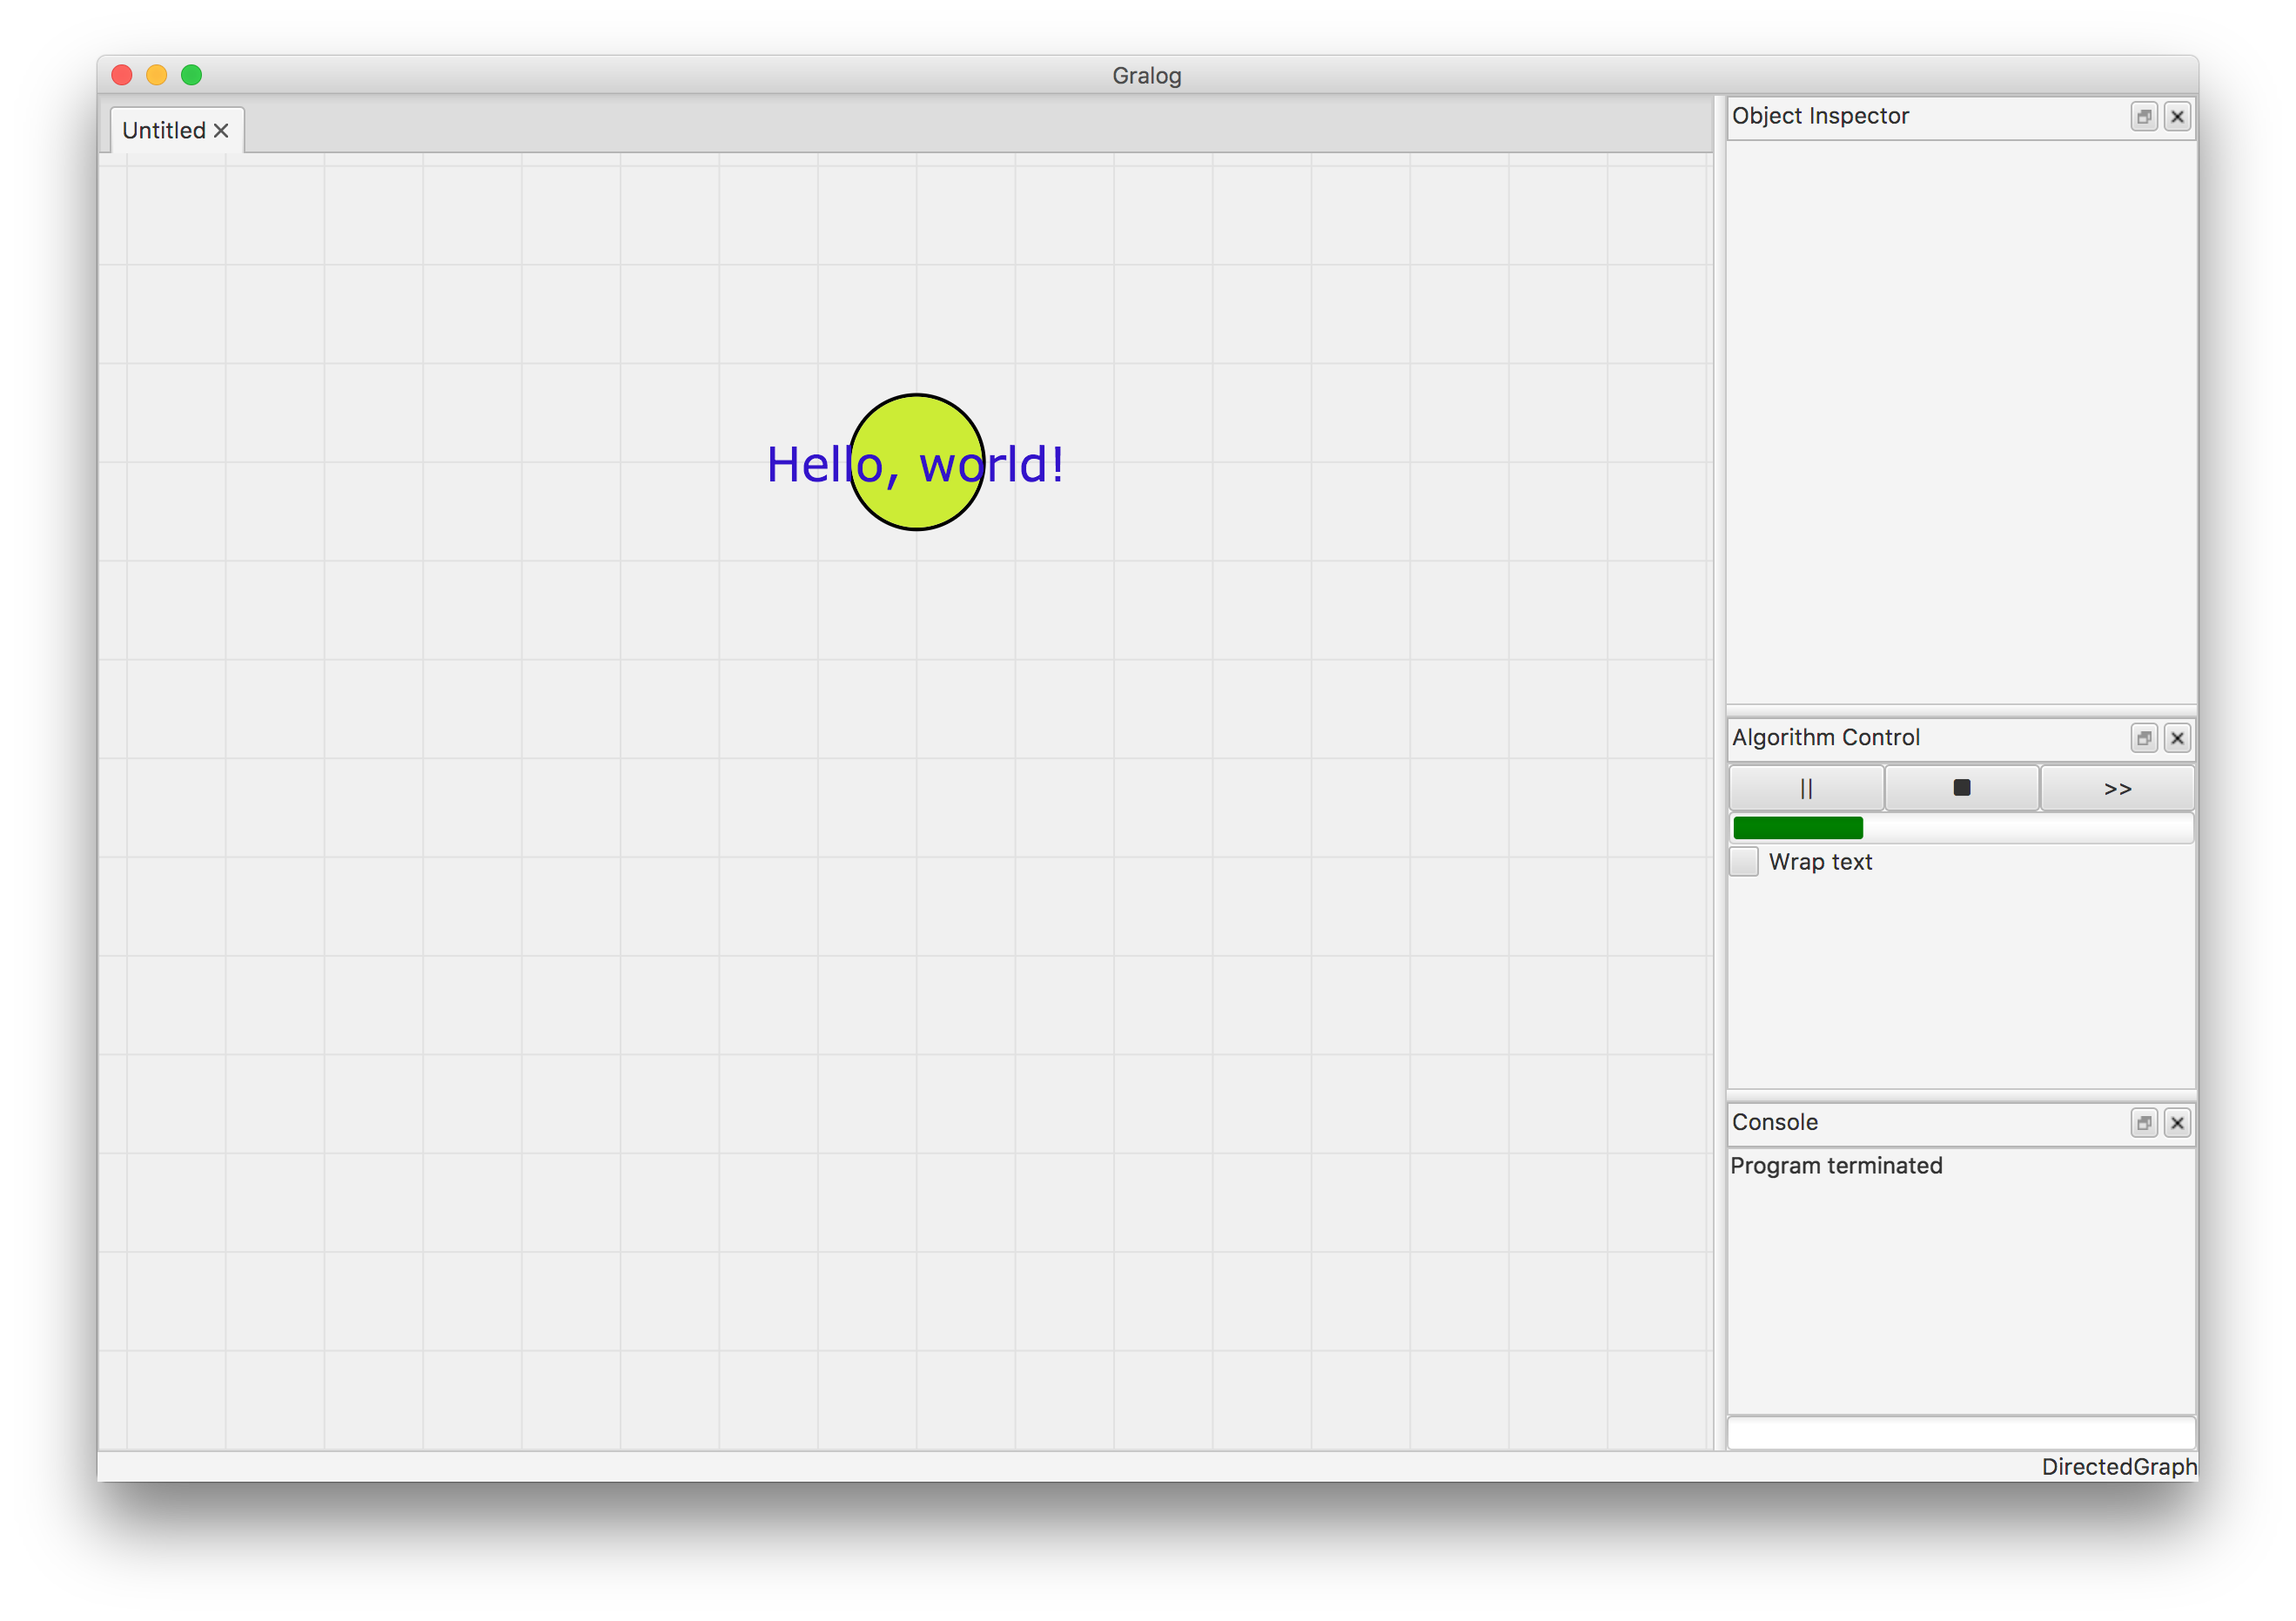
\includegraphics[width=\textwidth]{helloWorld.png}
\end{figure}


\subsection{Troubleshooting and Pro-Tips}
\subsection{Gralog Installation}
First obviously make sure you have python installed (version $\ge
2.7$). Also make sure that Gralog.py is in the directory as the file you
wish to execute. Obviously you can mess around with the file structure
to fit your needs but in this configuration they must be in the same
directory. For other outstanding problems feel free to shoot an email
at \texttt{gralog@tu-berlin.de} (TODO: make the email address.)

\subsection{A Good Rule}
Do not incorporate the "`hashtag"' symbol into variable names or messages. The \# symbol is reserved and using it may cause Gralog to misinterpret messages, which could result in spurious outcomes from your code.

\section{Introduction}
Now that you have the code running and set up, what will follow is a brief explanation of all of the functionality which we have built, structured in an intuitive manner.

\subsection{The Graph Class}
The first relevant class is Graph. In every program, you must choose a graph on which to execute your program. This is accomplished by instantiating the class Graph. 

\begin{lstlisting}
g = Graph();
\end{lstlisting}

In the constructor you specify which type of graph (directed,
undirected, a Kripke structure, a finite automaton, a Büchi automaton) you would like. No
argument means use the graph that is currently opened in Gralog, whatever (type) it may be.

The Graph class can be seen as the moderator of the program. You will use it to do all of the surface-level, more general commands pertaining to the graph itself. The more intricate details will be done using the following two:

\subsection{The Vertex Class}
Each vertex is represented as an object of the class Vertex. It is distinguished by its unique ID. 

\begin{lstlisting}
v = g.createVertex();
\end{lstlisting}

All methods pertaining to the individual vertices, such as their color, neighbours, or label, are most easily manipulated using methods of this class. For example:

\begin{lstlisting}
v = g.createVertex(id=42);
v.setLabel("f00");
neighbours = v.getNeighbours();
myLabel = v.getLabel();
v.delete();
\end{lstlisting}

\subsection{The Edge Class}
Each edge is represented as an object of hte Edge class. It is distinguished by its unique ID; however, in graphs without multi-edges, it can also be distinguished by its source and target vertices.

\begin{lstlisting}
e = g.createEdge(v1,v2,directed=False);
\end{lstlisting}

All methods pertaining to the individual edges, such as their color, adjacent edges, or label, are most easily manipulated using methods of this class. For example:

\begin{lstlisting}
e = g.createEdge(v1,v2,directed=False,id=451);
e.setLabel("f00");
adjacentEdges = e.getAdjacentEdges();
target = e.getTarget();
e.delete();
\end{lstlisting}

\subsection{Printing to the Console}
To print to the Gralog console, please use the method gPrint(str: message). Please note that this message must be a single-line string. No new-lines please!

\begin{lstlisting}
#!/usr/bin/python
#HelloWorld.py
from Gralog import *
g = Graph(None);
#end boiler plate

gPrint("hello world on the Gralog Console yeaaaahhh");
\end{lstlisting}

\section{Global Functions}
\begin{description}


\item[gPrint(String: message)] \emph{returns} \texttt{void}

Passes the message to Gralog to display in the console. Make sure this is in fact a string, or it will not work. Also please avoid new-lines/multiline messages, as they will not work.

Also: \textbf{PLEASE PLEASE PLEASE} do \textbf{not} use just \textbf{normal print} - this will crash the program immediately and you will be sad, and we will not be sympathetic because we explicitly warned that this may happen. :'(
\end{description}

\section{Class Vertex - Documentation}

\subsection{Instance Variables}
There are instance variables - however, they are not meant to be directly accessed by the user and are thus not detailed here.\\

\textbf{{\large Relevant Methods}}
\textit{Note: optional parameters are in square brackets}
\subsection{Manipulating Methods}
\begin{description}
\label{deleteVertexClass}\item[delete()] \emph{returns} \texttt{void}(corresponds to \textit{deleteVertex})\\
Deletes self from the graph.

\label{addEdgeClass}\item[connect(Vertex: v1, {[Integer: edgeId]})] \emph{returns} \texttt{Edge} (corresponds to \textit{addEdge})\\
Creates a new \texttt{Edge} object from self to \texttt{v1}. The directedness of the Edge will correspond to the type of Graph the edge is being added to (directed Graph $\to$ directed edge, automaton $\to$ transition, etc.). If un-directed, v.connect(v1) is equivalent to v1.connect(v). If no \texttt{edgeId}
is passed, a suitable id is chosen. If an id is passed that has
already been assigned, a suitable new one is silently chosen.

\label{getAllEdgesBetweenClass}\item[getAllEdgesBetween(Vertex: v1)] \emph{returns}\texttt{void} (corresponds to \textit{getAllEdgesBetween)}

Deletes all edges in the graph
between self and \texttt{v1} respecting
the direction if the graph has directed edges.
If no such edges exist, nothing happens.


\end{description}
\subsection{Getter Methods}
\begin{description}
\item[getId()] \emph{returns} \texttt{int}\\
Returns the id of self

\item[getLabel()] \emph{returns} \texttt{string}\\
Returns the label of self

\item[getFillColor()] \emph{returns} \texttt{string}\\
Returns the (fill) color of self, in the format that the user \textit{had} specified (hex or rgb).

\item[getColor()] \emph{returns} \texttt{string}\\
Same as getFillColor()

\item[getStrokeColor()] \emph{returns} \texttt{string}\\
Returns the stroke color of the \texttt{Vertex} object, in the format that the user \textit{had} specified (hex or rgb).

\item[get(String: property)] \emph{returns} \texttt{class specified by property}\\
Returns the value of \texttt{prop}. For example, v.get("label") would return a string. Possible values for \texttt{prop} are label, radius, fillColor, strokeColor, and shape, although the most common queried attributes have their own query methods. This is also useful if you wish to define your own vertex attributes in an extension of the Vertex class.

\label{getNeighboursClass}\item[getNeighbours()]\emph{returns}\texttt{list of Vertex objects}\quad(corresponds to \textit{getNeighbours})


Returns a list of all the vertices connected to self, regardless of direction.

\label{getOutgoingNeighboursClass}\item[getOutgoingNeighbours()]\emph{returns} \texttt{list of Vertex objects}\quad(corresponds to \textit{getOutgoingNeighbours})

Returns a list of all the vertices v' such that there is an edge from self to v' in directed graphs (equivalent to getNeighbours in undirected graphs)

\label{getIncomingNeighboursClass}\item[getIncomingNeighbours()]\emph{returns} \texttt{list of Vertex objects}\quad(corresponds to \textit{getIncomingNeighbours})

Returns a list of all the vertices v' such that there is an edge from v' to self in directed graphs (equivalent to getNeighbours in undirected graphs)

\label{getIncidentEdgesClass}\item[getIncidentEdges()]\emph{returns} \texttt{list of Edge objects}\quad(corresponds to \textit{getIncidentEdges})


Returns a list of all the Edges e with an endpoint at self, regardless of their direction.

\item[getOutgoingEdges()]\emph{returns}
  \texttt{list of Edge objects}

Returns a list of all the Edges e with an \textit{source Vertex} = self.

\label{getIncomingEdgesClass}\item[getIncomingEdges()]\emph{returns} \texttt{list of Edge objects}\quad(corresponds to \textit{getIncomingEdges})

Returns a list of all the Edges e with an \textit{target Vertex} = self.

\end{description}
\subsection{Setter Methods}
\begin{description}
\label{setVertexLabelClass}\item[setLabel(String: label)]\emph{returns} \texttt{void}\\\quad(corresponds to \textit{setVertexLabel})

Sets the vertex's label.

\label{setVertexRadiusClass}\item[setRadius(float: radius)] \emph{returns}\texttt{void}(corresponds to \textit{setVertexR})

Sets the radius (ie width and height) of self to \texttt{radius}.

\item[setHeight(float: height)] \emph{returns}
  \texttt{void}

Sets the height of self to \texttt{height}.

\label{setVertexShapeClass}\item[setShape(String: shape)] \emph{returns} \texttt{void}\quad(corresponds to \textit{setVertexShape})


Sets the shape of self to \texttt{shape}. Currently supported shapes are ``ellipse",``diamond",and ``rectangle".

\item[setWidth(float: width)] \emph{returns}
  \texttt{void}

Sets the width of self to \texttt{width}. 

\hyperref[radiusWidthHeightDiagram]{\textit{An explanation of width, height, and radius}}

\item[setCoordinates((Integer,Integer): coordinates)]\emph{returns}
  \texttt{void}\\
Sets the vertex's coordinates to the coordinate pair passed. It is possible to specify only one of the two, for example by saying v.setCoordinates((None,42)); which sets the vertex's y coordinate to 42 and doesn't affect the x coordinate.

\label{setVertexFillColorClass}\item[setFillColor({[string: colorHex]},{[(int,int,int): colorRGB]})]\emph{returns}
  \texttt{void} (corresponds to \textit{setVertexFillColor})

Sets the \textit{fill} colour to the Hex code colour
specified as a string or the RGB colour specified. colorHex can also be
a string of a common colour, such as \texttt{"red"} or
\texttt{"green."} \hyperref[colorNamesSupportedByGralog]{Full list of gralog supported color names}

Note that one of the two optional color parameters \textit{must} be filled, and both of them \textit{cannot} be filled.

\hyperref[colorNamesSupportedByGralog]{Color setting example}

\item[setColor({[string: colorHex]},{[(int,int,int): colorRGB]})]\emph{returns}
  \texttt{void}
  
Same as setFillColor

\label{setVertexStrokeColorClass}\item[setStrokeColor({[int: colorHex]},{[(int,int,int): colorRGB]}))] \emph{returns} \texttt{void} (corresponds to \textit{setVertexStrokeColor})

Sets the \textit{stroke} colour to the Hex code colour
specified as a string or the RGB colour specified. colorHex can also be
a string of a common colour, such as \texttt{"red"} or
\texttt{"green."} \hyperref[colorNamesSupportedByGralog]{Full list of gralog supported color names}

Note that one of the two optional color parameters \textit{must} be filled, and both of them \textit{cannot} be filled.

\hyperref[colorNamesSupportedByGralog]{Color setting example}

\item[\textbf{*}setVertexRadius(Vertex: v, float: radius)] \emph{returns}\texttt{void}\quad \hyperref[setVertexRadiusClass]{\textit{See proper method}}


Sets the radius (ie width and height) of the given vertex shape to \texttt{radius}.

\item[setVertexHeight(Vertex: v, float: height)] \emph{returns}
  \texttt{void}

Sets the height of the given vertex to \texttt{height}.

\item[setVertexWidth(Vertex: v, float: width)] \emph{returns}
  \texttt{void}
  
\label{setVertexPropertyClass}\item[setProperty(String: propertyName, String: propertyValue)] \emph{returns} \texttt{void}\quad(corresponds to \textit{setVertexProperty})

Sets self's attribute specified by \texttt{propertyName} to the value in \texttt{propertyValue}. Be careful using this method! If you can, use the pre-programmed methods instead.

Sets the width of the given vertex to \texttt{width}. 

\hyperref[radiusWidthHeightDiagram]{\textit{An explanation of width, height, and radius}}

\end{description}

\section{Class Edge - Documentation}

\subsection{Instance Variables}
There are instance variables - however, they are not meant to be directly accessed by the user and are thus not detailed here.\\

\textbf{{\large Relevant Methods}}
\textit{Note: optional parameters are in square brackets}
\subsection{Manipulating Methods}
\begin{description}
\label{deleteEdgeClass}\item[delete()] \emph{returns} \texttt{void} (corresponds to \textit{deleteEdge})\\
Deletes self from the graph.



\end{description}
\subsection{Getter Methods}
\begin{description}
\item[getId()] \emph{returns} \texttt{int}\\
Returns the id of self

\label{getEdgeLabelClass}\item[getLabel()] \emph{returns} \texttt{string}\quad(corresponds to \textit{getEdgeLabel})\\
Returns the label of self

\label{getEdgeWeightClass}\item[getWeight()] \emph{returns} \texttt{float}\quad(corresponds to \textit{getEdgeWeight})
\\
Returns the weight of self


\label{getEdgePropertyClass}\item[get(String: property)] \emph{returns} \texttt{class specified by property}\quad(corresponds to \textit{getEdgeProperty})\\
Returns the value of \texttt{prop}. For example, e.get("label") would return a string. Possible values for prop are label, weight, isDirected, thickness, color, type, and edge-Type, although the most common queried attributes have their own query methods. This is also useful if you wish to define your own vertex attributes in an extension of the Vertex class.

\item[getColor()] \emph{returns} \texttt{string}\\
Returns the color of self, in the format that the user \textit{had} specified (hex or rgb).

\item[getSource()] \emph{returns} \texttt{Vertex}\\
Returns the source endpoint of self

\item[getTarget()] \emph{returns} \texttt{Vertex}\\
Returns the target endpoint of self

\item[get(String: property)] \emph{returns} \texttt{class specified by property}\\
Returns the value of \texttt{prop}. For example, e.get("label") would return a string. Possible values for \texttt{prop} are label, radius, fillColor, strokeColor, and shape, although the most common queried attributes have their own query methods. This is also useful if you wish to define your own vertex attributes in an extension of the Vertex class.

\item[getProperty(String: property)] \emph{returns} \texttt{class specified by property}\\
Returns the value of \texttt{prop}. 
Same as \textit{get(String: property)}

\item[getAdjacentEdges()]\emph{returns}
  \texttt{list of Edge objects}

Returns a list of all the Edges that share an endpoint with self.

\end{description}
\subsection{Setter Methods}
\begin{description}
\label{setEdgeLabelClass}\item[setLabel(String: label)]\emph{returns} \texttt{void}\\\quad(corresponds to \textit{setEdgeLabel})

Sets the vertex's label.

\label{setEdgeContourClass}\item[setContour(str: contour)] \emph{returns} \texttt{void}\quad(corresponds to \textit{setEdgeContour})

Sets the contour of passed self. Possible values are
\texttt{"dashed"}, \texttt{"dotted"}, \texttt{"plain"}.

\label{setEdgeColorClass}\item[setColor({[string: colorHex]},{[(int,int,int): colorRGB]})]\emph{returns} \texttt{void}\quad(corresponds to \textit{setEdgeColor})
Sets the colour to the Hex code colour
specified as a string or the RGB colour specified. colorHex can also be
a string of a common colour, such as \texttt{"red"} or
\texttt{"green."} \hyperref[colorNamesSupportedByGralog]{Full list of gralog supported color names}

Note that one of the two optional color parameters \textit{must} be filled, and both of them \textit{cannot} be filled.

\hyperref[colorNamesSupportedByGralog]{Color setting example}

\label{setEdgeWeightClass}\item[setWeight({float: weight})]\emph{returns} \texttt{void}\quad(corresponds to \textit{setEdgeWeight})

Set's the weight of self to the given weight.

\label{setEdgeThiccnessClass}\item[setThickness({float: weight})]\emph{returns} \texttt{void}\quad(corresponds to \textit{setEdgeThickness})

Set's the thickness of the line of self to the given thickness.

\label{setEdgePropertyClass}\item[setProperty(String: propertyName, String: propertyValue)] \emph{returns} \texttt{void}\quad(corresponds to \textit{setEdgeProperty})

Sets self's attribute specified by \texttt{propertyName} to the value in \texttt{propertyValue}. Be careful using this method! If you can, use the pre-programmed methods instead.
\end{description}
\section{Class Graph}

\subsection{Instance Variables}


\begin{longtable}{p{\q}p{\q}}
Instance Variable & Meaning and Usage \\ \hline
\textbf{Dictionary} \textit{vertices} & A dictionary that holds all of the Vertex objects known to the graph. This should ideally not be changed by the programmer. \\\hline
\textbf{Dictionary} \textit{edges} & A dictionary that holds all of the Edge objects known to the graph. This should ideally not be changed by the programmer. \\\hline
\textbf{Integer} \textit{id} & The id of the graph that is used in communication with gralog. This should ideally not be changed by the programmer. \\ \hline
\textbf{Dictionary} \textit{variablesToTrack} & Objects in format (name,value). These are displayed in the Algorithm Control Panel. These may be changed. \\ \hline
\textbf{Dictionary} \textit{variablesToTrack} & Objects in format (name,value). These are displayed in the Algorithm Control Panel. These may be changed. \\ \hline
\end{longtable}


\textbf{{\large Relevant Methods}}
\textit{Note: optional parameters are in square brackets}


\begin{description}
\item[Graph({[str: format]})] \emph{returns} a Graph Object.\\\\
This is the constructor for the Graph class. It returns one of two things, depending on the parameter passed. If None is passed as the parameter, then \textit{no new graph is created}. Rather, the graph that is currently open in Gralog is passed to your program and a reference to it is stored in the Graph object. This Graph object now also contains all relevant (rudimentary) features of the open graph. The other parameter options are:
\begin{itemize}
\item nothing, e.g.\@ \texttt{g = Graph()}, (this is the default, which is interpreted as ''undirected")
\item \texttt{"{}undirected"},
\item \texttt{"directed"},
\item \texttt{"buechi"},
\item \texttt{"kripke"},
\item \texttt{"{}automaton"}.
\end{itemize}
\end{description}

Use of these parameters causes Gralog to create a new (empty) graph of the requested type, a reference to which is then passed back to your program and stored in the returned Graph object.
\subsection{Graph Manipulating Methods}
\textbf{Note:} every time a \texttt{Vertex} object is a function \textit{parameter}, the programmer may pass \textit{either} a \texttt{Vertex} object \textit{or} a valid vertex id; likewise for \texttt{Edge} objects as parameters and edge id's. In order to avoid redundancy, there are not duplicate method descriptions.\\\\
\textbf{Another Note:} vertex/edge manipulating methods (such as getting/setting label or some other attribute) can be done using the following methods. However, they are actually not designed to be directly used. Rather, you must use the methods in the Vertex and Edge classes that correspond to each. If you do use these methods directly, it may cause inconsistency between python and Gralog, leading to avoidable conundra and discontent. Corresponding methods are linked, and methods to be avoided are marked with a \textbf{*}.

\begin{description}
\item[addVertex({[int: vertexId]}{[(double, double): pos]})]\emph{returns}
  \texttt{Vertex} object

  Creates a new \texttt{Vertex} object. If both coordinates coordinates in coordinate Vector \texttt{(x\_coord,y\_coord)} are \textit{not} passed,
  random coordinates are chosen
  %and the vertex is selected in
  %the Gralog UI.
  If no \texttt{vertexId} is passed, a suitable id is
  chosen by Gralog automatically. If an id is passed that has already
  been assigned, a suitable new one is silently chosen.
  
  The \texttt{vertex} returned has the final id assigned to it.
  
  \hyperref[addVertexExample]{Example}

  
\item[\textbf{*}deleteVertex(Vertex: v)] \emph{returns} \texttt{void}\quad \hyperref[deleteVertexClass]{\textit{See proper method}}

Deletes the given vertex from the graph. If the vertex does not exist, the program continues\footnote{you will however receive a warning message in the console \label{deleteVertexWarning}}


\item[\textbf{*}addEdge(Vertex: source, Vertex target,{[int: egdeId]})] \emph{returns} \texttt{Edge} object\quad \hyperref[addEdgeClass]{\textit{See proper method}}


Creates a new \texttt{Edge} object from the source vertex to the
target vertex. The directedness of the Edge will correspond to the type of Graph the edge is being added to (directed Graph $\to$ directed edge, automaton $\to$ transition, etc.). If un-directed, the
order of target and source vertex is irrelevant. If no \texttt{edgeId}
is passed, a suitable id is chosen. If an id is passed that has
already been assigned, a suitable new one is silently chosen.


\item[\textbf{*}deleteEdge(Edge: e)] \emph{returns} \texttt{void}\quad \hyperref[deleteEdgeClass]{\textit{See proper method}}

Deletes the edge from the graph. If the edge does not exist, nothing
happens.\textsuperscript{\ref{deleteVertexWarning}}


\item[deleteEdge((Vertex,Vertex): edge)] \emph{returns} \texttt{void} \footnote{make sure this is actually a tuple, or it will not work! Also note vertices and vertex id's can be mixed and matched, should that be practical, such that you could call g.edgeMethodFoo((Vertex,id)) or g.edgeMethodFoo((id,Vertex)) and they would be equivalent \label{makeSureATupleWarning1}}

  Deletes the edge with the greatest id from the list of all edges
  between the vertex in the first position of the tuple \texttt{edge} and the vertex which is the second position in tuple \texttt{source} respecting
  the direction if the graph has directed edges. If no such edge exists, nothing happens.


%\item[deleteEdge((int,int): edge)] \emph{returns}
%  \texttt{Boolean} \textsuperscript{\ref{makeSureATupleWarning1}}

  %Deletes the edge with the greatest id from the list of all edges
%  between the vertex whose \texttt{id} is the first element of tuple \texttt{edge}, and the vertex whose \texttt{id} is the second element of tuple \texttt{source} respecting
%  the direction if the graph has directed edges. If no such edge exists, nothing happens.

\item[existsEdge((Vertex,Vertex): edge)] \emph{returns}
  \texttt{void} \textsuperscript{\ref{makeSureATupleWarning1}}

  Returns whether there exists an edge between the first vertex of the tuple \texttt{edge} and the second (or from the first to the second in directed graphs).
  
  
\item[existsEdge(Edge: edge)] \emph{returns}
  \texttt{Boolean}

  Returns whether that specified edge (ie. the one with ID associated with the object) currently exists in the specified graph in Gralog. 
  
%\item[existsEdge(int: id)] \emph{returns}
%  \texttt{boolean}

%  Returns whether an edge with specified id currently exists in the specified graph in Gralog. 
  
\item[existsVertex(Vertex: vertex)] \emph{returns}
  \texttt{Boolean}

  Returns whether that specified Vertex (ie. the one with ID associated with the object) currently exists in the specified graph in Gralog. 
  
%\item[existsVertex(int: id)] \emph{returns}
%  \texttt{boolean}

%  Returns whether a Vertex with specified id currently exists in the specified graph in Gralog. 


\item[\textbf{*}getAllEdgesBetween((Vertex,Vertex): vertexPair)] \emph{returns} \texttt{void}\quad \hyperref[getAllEdgesBetweenClass]{\textit{See proper method}}

  Returns all edges in the graph
  between the vertex in the first position of the tuple \texttt{vertexPair} and the vertex which is the second position in tuple \texttt{vertexPair} respecting
  the direction if the graph has directed edges.
  If no such edges exist, nothing happens.
  
%\item[deleteAllEdges((int,int): vertexPair)] \emph{returns}
%  \texttt{void}

%  Deletes all edges
%  between the vertex whose \texttt{id} is the first element of tuple \texttt{edge}, and the vertex whose \texttt{id} is the second element of tuple \texttt{source} respecting
%  the direction if the graph has directed edges. If no such edges exist, nothing happens.
  
\end{description}

\subsection{Setter Functions}
\begin{description}
\item[\textbf{*}setVertexFillColor(Vertex: v,{[string: colorHex]},{[(int,int,int): colorRGB]})]\emph{returns}\texttt{void}\quad \hyperref[setVertexFillColorClass]{\textit{See proper method}}

Sets the \textit{fill} colour of the given \texttt{Vertex} to the Hex code colour
specified as a string or the RGB colour specified. colorHex can also be
a string of a common colour, such as \texttt{"red"} or
\texttt{"green."} \hyperref[colorNamesSupportedByGralog]{Full list of gralog supported color names}

Note that one of the two optional color parameters \textit{must} be filled, and both of them \textit{cannot} be filled.

\hyperref[colorNamesSupportedByGralog]{Color setting example}

\item[\textbf{*}setVertexStrokeColor(Vertex: v,{[string: colorHex]},{[(int,int,int): colorRGB]}))] \emph{returns} \texttt{void}\quad \hyperref[setVertexStrokeColorClass]{\textit{See proper method}}

Sets the \textit{stroke} colour of the given \texttt{Vertex} to the Hex code colour
specified as a string or the RGB colour specified. colorHex can also be
a string of a common colour, such as \texttt{"red"} or
\texttt{"green."} \hyperref[colorNamesSupportedByGralog]{Full list of gralog supported color names}

Note that one of the two optional color parameters \textit{must} be filled, and both of them \textit{cannot} be filled.

\hyperref[colorNamesSupportedByGralog]{Color setting example}

\item[\textbf{*}setEdgeContour(Edge: edge, str: contour)] \emph{returns}\texttt{void}\quad \hyperref[setEdgeContourClass]{\textit{See proper method}}

Sets the contour of passed \texttt{Edge}. Possible values are
\texttt{"dashed"}, \texttt{"dotted"}, \texttt{"plain"}.

\item[\textbf{*}setEdgeColor(Edge: v, {[string: colorHex]},{[(int,int,int): colorRGB]}))] \emph{returns} \texttt{void}\quad \hyperref[setEdgeColorClass]{\textit{See proper method}}

Sets the colour of the given \texttt{Edge} to the Hex code colour
specified as a string or the RGB colour specified. colorHex can also be
a string of a common colour, such as \texttt{"red"} or
\texttt{"green."} \hyperref[colorNamesSupportedByGralog]{Full list of gralog supported color names}

Note that one of the two optional color parameters \textit{must} be filled, and both of them \textit{cannot} be filled.

\hyperref[colorNamesSupportedByGralog]{Color setting example}



  
\item[setVertexDimension(Vertex: v, float: width, str: dimension)]\emph{returns} \texttt{void}

Sets the dimension of the given vertex to the dimension specified. This functionality is primarily useful for non-standard shapes, if you were to extend gralog to include such a thing. Other than in this case, it is recommended that you use the built-in functions.

\item[\textbf{*}setVertexShape(Vertex: v, str: shape)] \emph{returns} \texttt{void}\quad \hyperref[setVertexShapeClass]{\textit{See proper method}}


Sets the given vertex to be the specified shape. Currently supported
are ``\texttt{ellipse"}, \texttt{"diamond"}, and \texttt{"rectangle"}.

\item[\textbf{*}setEdgeWeight(Edge: e, float: weight)] \emph{returns} \texttt{void}\quad \hyperref[setEdgeWeightClass]{\textit{See proper method}}


Sets edge weight to \texttt{weight}. Not to be confused with setEdgeThickness

\item[\textbf{*}setEdgeThickness(Edge: e, float: thickness)] \emph{returns} \texttt{void}\quad \hyperref[setEdgeThiccnessClass]{\textit{See proper method}}


Sets edge thickness to \texttt{thickness}. Not to be confused with setEdgeWeight

\item[\textbf{*}setEdgeProperty(Edge: edge, String: propertyName, String: propertyValue)] \emph{returns} \texttt{void}\quad \hyperref[setEdgePropertyClass]{\textit{See proper method}}


Sets \texttt{edge}'s attribute specified by \texttt{propertyName} to the value in \texttt{propertyValue}.

\item[\textbf{*}setVertexProperty(Vertex: vertex, String: propertyName, String: propertyValue)] \emph{returns} \texttt{void}\quad \hyperref[setVertexPropertyClass]{\textit{See proper method}}


Sets \texttt{vertex}'s attribute specified by \texttt{propertyName} to the value in \texttt{propertyValue}.

\item[\textbf{*}setVertexLabel(Vertex: v, str: label)] \emph{returns} \texttt{void}\quad \hyperref[setVertexLabelClass]{\textit{See proper method}}

Sets the edge's label to the \texttt{label}

\item[\textbf{*}setEdgeLabel(Edge: v, str: label)] \emph{returns} \texttt{void}\quad \hyperref[setEdgeLabelClass]{\textit{See proper method}}

Sets the vertex's label to the \texttt{label}
  
\end{description}

\subsection{Getter Functions}
\begin{description}
\item[getGraph(str: graphFormat)]\emph{returns}
  \texttt{str}

Returns a string representation of the graph. Several formats are supported: GraphXML (parameter "XML"), TikZ (parameter "tikz"), Trivial Graph Format (paramter "TGF"), and Gralog Trivial Graph Format (pamater "GTGF"). \hyperref[graphFormatsInDetail]{Read more about them here}.

This is useful in at least the following two scenarios: 1: to take the graph Gralog has given, and import it into an external library for processing there (such as NetworkX, or TODO: another popular library). 2: to copy the contents of one graph into another Gralog graph. \hyperref[getGraphExample]{See an example here}.


\item[getVertices()]\emph{returns}
  \texttt{list of Vertex objects}

Returns a list of all the vertices in the graph.

\item[getAllVertices()]

  The same as \texttt{getVertices()}.


\item[getEdges()]\emph{returns}
  \texttt{list of Edge objects}

\item[getAllEdges()]

  The same as \texttt{getEdges()}.

  
Returns a list of all the edges graph.

\item[\textbf{*}getNeighbours(Vertex: vertex)]\emph{returns} \texttt{list of Vertex objects}\quad \hyperref[getNeighboursClass]{\textit{See proper method}}

Returns a list of all the vertices connected to \texttt{vertex}, regardless of direction.

\item[\textbf{*}getOutgoingNeighbours(Vertex: vertex)]\emph{returns} \texttt{list of Vertex objects}\quad \hyperref[getOutgoingNeighboursClass]{\textit{See proper method}}

Returns a list of all the vertices v' such that there is an edge from \texttt{vertex} to v' in directed graphs (equivalent to getNeighbours in undirected graphs)

\item[\textbf{*}getIncomingNeighbours(Vertex: vertex)]\emph{returns} \texttt{list of Vertex objects}\quad \hyperref[getIncomingNeighboursClass]{\textit{See proper method}}

Returns a list of all the vertices v' such that there is an edge from v' to \texttt{vertex} in directed graphs (equivalent to getNeighbours in undirected graphs)

\item[\textbf{*}getIncidentEdges(Vertex: vertex)]\emph{returns} \texttt{list of Edge objects}\quad \hyperref[getIncidentEdgesClass]{\textit{See proper method}}


Returns a list of all the Edges e with an endpoint at \texttt{vertex}, regardless of their direction.

\label{getOutgoingEdgesClass}\item[getOutgoingEdges(Vertex: vertex)]\emph{returns} \texttt{list of Edge objects}\quad(corresponds to \textit{getOutgoingEdges})

Returns a list of all the Edges e with an \textit{source Vertex} = \texttt{vertex}.

\item[getIncomingEdges(Vertex: vertex)]\emph{returns} \texttt{list of Edge objects}

Returns a list of all the Edges e with an \textit{target Vertex} = \texttt{vertex}.

\item[getAdjacentEdges(Edge: edge)]\emph{returns}
  \texttt{list of Edge objects}

Returns a list of all the Edges e' that share an endpoint with \texttt{edge}.

\item[\textbf{*}getEdgeWeight(Edge: edge)]\emph{returns} \texttt{float}\quad \hyperref[getEdgeWeightClass]{\textit{See proper method}}

Returns the weight of \texttt{edge}.

\item[\textbf{*}getEdgeLabel(Edge: edge)]\emph{returns} \texttt{string}\quad \hyperref[getEdgeLabelClass]{\textit{See proper method}}

Returns the label of \texttt{edge}.

\item[\textbf{*}getEdgeProperty(Edge: edge, String: prop)]\emph{returns} \texttt{type of prop}\quad \hyperref[getEdgePropertyClass]{\textit{See proper method}}

Returns the value of \texttt{prop} in the passed \texttt{Edge}. For example, g.getEdgeProperty(e1,"weight") would return a float. Possible values for \texttt{prop} are label, weight, isDirected, thickness, color, type, and edgeType, although the most common queried attributes have their own query methods. This is also useful if you wish to define your own edge attributes in an extension of the Edge class.

\item[getVertexProperty(Vertex: vertex, String: prop )]\emph{returns}
  \texttt{class specified by prop}

Returns the value of \texttt{prop} in the passed \texttt{Vertex}. For example, g.getVertex(v1,"label") would return a string. Possible values for \texttt{prop} are label, radius, fillColor, strokeColor, and shape, although the most common queried attributes have their own query methods. This is also useful is you wish to define your own vertex attributes in an extension of the Vertex class.

{\Large End: private!}

\item[requestVertex()]\emph{returns}
  \texttt{Vertex}\\
Waits for user to click a vertex, then returns the vertex that the user clicks on. 

\item[requestRandomVertex()]\emph{returns}
  \texttt{Vertex}\\
Chooses a random vertex from the graph.

\item[requestEdge()]\emph{returns}
  \texttt{Edge}\\
Waits for user to click a edge, then returns the edge that the user clicks on. 

\item[requestRandomEdge()]\emph{returns}
  \texttt{Edge}\\
Chooses a random edge from the graph.

\item[requestInteger()]\emph{returns}
  \texttt{Integer}\\
Waits for user to click a integer, then returns the integer that the user clicks on. 

\item[requestFloat()]\emph{returns}
  \texttt{Float}\\
Waits for user to click a float, then returns the float that the user clicks on. 

\item[requestString()]\emph{returns}
  \texttt{String}\\
Waits for user to click a string, then returns the string that the user clicks on. 

\end{description}

\subsection{Control Functions}
\begin{description}


\item[pause(String{[]}: *args)]\emph{returns}
  \texttt{void}\\
Waits for user to either press the space bar, or the ``play" icon in the Algorithm Control Panel. While paused, tracked variables are displayed in the Algorithm Control Panel. Optionally, in the args input, you can add the following options:
\begin{itemize}
    \item you can give, as the first parameter, the rank of the pause. In this way you can give the pauses a hierarchy. If during a pause of rank "n", you press the ``skip" button the Algorithm Control Panel, afterwards all pauses of rank n or higher will be ignored.
    \item You can add variables you would like to track individually in the moment, in the form of name-value \begin{lstlisting}
g.pause(("name1","val1"),("name2",var2),...("nameN",varN));
\end{lstlisting}
\end{itemize}

Either strings or variables can be passed as the value, and a string representation of the variables will be displayed by Gralog.

\item[track(String: name, Variable: var)]\emph{returns}
  \texttt{void}\\
Specifies variable \texttt{var} to be tracked under the name \texttt{name}. Whenever the script is programmatically paused (ie. not by just clicking the pause button), that key-value pair will be shown in its most updated form in the Algorithm Control Panel.\\

Word to the wise: if you pass an int, str, or other primitive-acting variable, the tracked value will not be updated as the variable itself it updated. In this case, you will have to re-track the variable (I'm sorry, but python is too high-level language to support integer pointers and the like). However, a Vertex, for example, being a pointer to an object in memory, will be displayed in its most updated form each time.


\item[unTrack(String: name)]\emph{returns}
  \texttt{void}\\
Disassociates the name \texttt{name} from any value it may be tracking. Now, if the script is programmatically paused, it will no longer be displayed with its former value.




A simple example for how to use variable Tracking \hyperref[varTrackingExample]{can be found here}.

\end{description}

\section{Code Examples}

\begin{description}
\item[addVertex({[int: vertexId]}{[(double: x\_coord, double: y\_coord)]})]\emph{returns}
  \texttt{Vertex} object


  \begin{example}
    \begin{lstlisting}[title={addVertex Example},label=addVertexExample]
    #!/usr/bin/python
    #HelloWorld.py
    from Gralog import *
    g = Graph(None);
    #end boiler plate
    
    v = g.addVertex(); #adds a vertex with a random id and random coordinates
    v.setLabel("v: " + str(v.getId()));#shows the id gralog assigned on the vertex in Gralog
    
    v1 = g.addVertex(420);
    v1.setLabel("v1: " + str(v1.getId()));
    
    v2 = g.addVertex((-10,2.2)); #adds a vertex at (0,2.2) and random id*
    v2.setLabel("v2: " + str(v2.getId()));
    
    v3 = g.addVertex(0,(11,-3)); #adds a vertex at (11,-3) with id=0
    v3.setLabel("v3: " + str(v3.getId()));
    
    g.pause();
    
    #now we try and add a new vertex with an id that is in use
    
    vDuplicate = g.addVertex(420);
    vDuplicate.setLabel("dup: " + str(vDuplicate.getId())); #it ends up not being 420
    
    \end{lstlisting}
    *technically this should be \texttt{v2 = g.addVertex(pos=(0,2.2))}; however, in order to make it user friendly the library allows for the user to misuse parameters in order to preserve clarity and brevity
  \end{example}

\item[Color Setting examples]


  \begin{example}
    \begin{lstlisting}[title={Color Setting Example},label=colorSettingExample]
    #!/usr/bin/python
    #HelloWorld.py
    from Gralog import *
    g = Graph("directed");
    #end boiler plate
    
    v = g.addVertex();
    v.setColor("PUCE");
    g.pause();
    v.setColor(colorHex="123456");
    g.pause();
    v.setColor(colorRGB = (255,255,255));
    g.pause();
    v.setStrokeColor("red");
    g.pause();
    v.setStrokeColor("#101010");
    g.pause();
    v.setStrokeColor(colorRGB = (1,2,3));
    g.pause();
    v2 = g.addVertex();
    e = g.addEdge(v,v2);
    e.setColor("green");
    g.pause();
    e.setColor(colorHex="99999f");
    g.pause();
    e.setColor(colorRGB = (23,45,131));
    #the following will not work
    e.setColor((23,45,131));
    \end{lstlisting}
  \end{example}
  

\item[Color Setting examples]


  \begin{example}
    \begin{lstlisting}[title={getGraph Example},label=getGraphExample]
    #!/usr/bin/python
    #Showing how to load a graph from python into a string, then transfer it to another graph
    from Gralog import *
    g = Graph("directed");
    g2 = Graph("directed");
    #end boiler plate
    
    #populate g with 10 vertices in random locations
    for x in range(10):
      g.addVertex();
    
    gString = g.getGraph("GTGF");#load g into a string
    g2.setGraph("GTGF",gString);#set g2 to graph isomorphic to g
    \end{lstlisting}
  \end{example}
  
\item[Variable Tracking Example]


  \begin{example}
    \begin{lstlisting}[title={Variable Tracking Example},label=varTrackingExample]
    #!/usr/bin/python
    #TrackingExample.py
    from Gralog import *
    g = Graph("directed");
    
    vertices=[];
    g.track("vertices",vertices);
    for x in range(5):
      v = g.addVertex();
      v.setLabel("v" + str(x));
      vertices.append(v);
    g.pause();#the array with the vertices will be displayed
    g.unTrack("vertices");
    for x in vertices:
      g.track("label of vertex "+str(x),x.getLabel());
    g.pause();#each vertex will be displayed with its label
    
    g.pause(("hello","world"));#each vertex, as well as the pair "hello","world" will be displayed

    \end{lstlisting}
  \end{example}
\end{description}

\begin{figure}[H]
\title{An explanation of the width, height, and radius properties of a \texttt{Vertex} object}
\label{radiusWidthHeightDiagram}
\centering
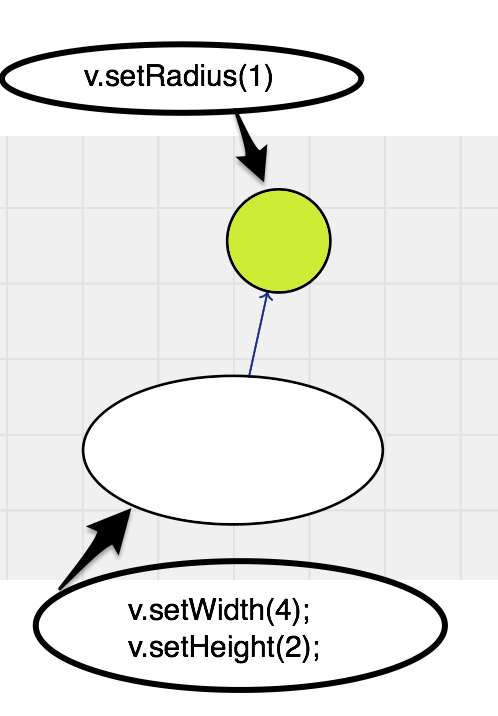
\includegraphics[width=200pt]{radiusWidthHeightDiagram.png}
\end{figure}


\begin{table}[h!]
  \begin{center}
    \caption{Color Names supported by Gralog}
    \label{colorNamesSupportedByGralog}
    \begin{tabular}{c|c} % <-- Alignments: 1st column left, 2nd middle and 3rd right, with vertical lines in between
      \textbf{Gralog color name} & \textbf{Hex Value}\\
      WHITE   &\#FFFFFF\\
\hline
BLACK   &\#000000\\
\hline
BLUE    &\#0000FF\\
\hline
GREEN   &\#00FF00\\
\hline
RED     &\#FF0000\\
\hline
GRAY    &\#808080\\
\hline
YELLOW  &\#FFFF00\\
\hline
CYAN    &\#00FFFF\\
\hline
MAGENTA &\#FF00FF\\
\hline
SILVER  &\#C0C0C0\\
\hline
MAROON  &\#800000\\
\hline
OLIVE &\#808000\\
\hline
DARK GREEN &\#008000\\
\hline
PURPLE  &\#800080\\
\hline
TEAL  &\#008080\\
\hline
NAVY    &\#000080\\
\hline
ORANGE  &\#FF4500
    \end{tabular}
  \end{center}
\end{table}

\subsection{Graph formats in detail}
\label{graphFormatsInDetail}
The four graph formats Gralog supports are the following: \href{https://en.wikipedia.org/wiki/GraphML}{GraphML}, \href{https://en.wikipedia.org/wiki/Trivial\_Graph\_Format}{Trivial Graph Format}, \href{https://en.wikipedia.org/wiki/PGF/TikZ}{TikZ}, and Gralog Trivial Graph Format. The first three are cross-platform compatible with other libraries, and can be imported and exported easily with the Gralog Python library. The last is primarily useful for intra-gralog communication. It is a simple extension of TGF, that introduces edge id's in the format. This allows simple graphs to be passed between the Gralog Python programs and Gralog without losing any basic data that cannot be retrieved. The locations, colors, labels, weights etc. are not preserved in this format (hence trivial) but for simple uses it is quick and practical.

\end{document}






\end{document}


%%% Local Variables:
%%% mode: latex
%%% TeX-master: t
%%% End:
